\documentclass[10pt,a4paper]{article}

\usepackage[margin=0.92in]{geometry}
\linespread{1.03}
\usepackage[T1]{fontenc}
\usepackage[utf8]{inputenc}
\usepackage{lmodern}
\usepackage{microtype}
\usepackage{amsmath,amssymb,amsthm}
\usepackage{booktabs}
\usepackage{array}
\usepackage{tabularx}
\usepackage{enumitem}
\usepackage{titlesec}
\usepackage[font=small,labelfont=bf,labelsep=period]{caption}
\usepackage{xcolor}
\usepackage{tikz}
\usetikzlibrary{arrows.meta,positioning,calc}
\usepackage[ruled,vlined,linesnumbered]{algorithm2e}
\usepackage[colorlinks=true,linkcolor=blue!55!black,citecolor=blue!55!black,urlcolor=blue!55!black]{hyperref}

\definecolor{tierzero}{HTML}{1B7F79}
\definecolor{tierone}{HTML}{C84B31}
\definecolor{mcpblue}{HTML}{2B4C7E}
\definecolor{slate}{HTML}{4A5568}
\definecolor{softbg}{HTML}{F7FAFC}
\definecolor{trackbg}{HTML}{EDF2F7}

\newtheorem{proposition}{Proposition}
\newtheorem{definition}{Definition}

\newcolumntype{Y}{>{\raggedright\arraybackslash}X}
\newcommand{\DelayAcct}{\texttt{DELAY1111\allowbreak\dots}}
\newcommand{\DelaySym}{\mathsf{DELAY}}
\newcommand{\SortTxs}{\textsc{SortTxs}}
\newcommand{\SelectTxs}{\textsc{SelectTxs}}
\newcommand{\NewCon}{\text{NewCon}}

\titlespacing*{\section}{0pt}{1.35ex plus 0.3ex minus 0.2ex}{0.6ex plus 0.15ex}
\titlespacing*{\subsection}{0pt}{1.0ex plus 0.25ex minus 0.15ex}{0.45ex plus 0.1ex}
\titlespacing*{\paragraph}{0pt}{0.75ex plus 0.2ex minus 0.1ex}{0.6em}

\setlength{\parskip}{0.28em}
\setlength{\parindent}{1.15em}
\setlength{\textfloatsep}{10pt plus 2pt minus 2pt}
\setlength{\floatsep}{8pt plus 2pt minus 2pt}
\setlength{\intextsep}{8pt plus 2pt minus 2pt}
\setlength{\abovedisplayskip}{6pt plus 2pt minus 2pt}
\setlength{\belowdisplayskip}{6pt plus 2pt minus 2pt}

\begin{document}

% ==================== PAGE 1: TITLE & ABSTRACT ====================
\begin{titlepage}
\centering
\vspace*{2.5cm}

{\LARGE\bfseries CU-Free Application-Controlled Execution\\[0.22em]
for New Constellation\par}
\vspace{0.65cm}
{\large\color{slate} Maker-Friendly Taker Speed Bumps Without Compute Unit Metering\par}
\vspace{1.05cm}
\begin{tabular}{@{}c@{\hspace{3.2cm}}c@{}}
{\large\bfseries Cavey Cool} & {\large\bfseries Frank} \\[0.22em]
{\normalsize\color{slate} Chief Science Officer} & {\normalsize\color{slate} Deputy Science Officer}
\end{tabular}\par
\vspace{0.35cm}
{\normalsize Temporal\par}
\vspace{0.6cm}
{\normalsize Supplementary Technical Note\par}
\vspace{0.2cm}
{\normalsize November 20, 2026\par}

\vspace{1.5cm}
\rule{0.86\textwidth}{0.5pt}
\vspace{0.6cm}

\begin{minipage}{0.84\textwidth}
\begin{center}
{\normalsize\bfseries Abstract}
\end{center}
\vspace{0.25em}
\small\noindent
\emph{New Constellation} (\NewCon)~\cite{KW26c} extends Solana's Alpenglow consensus with $k$ concurrent proposers whose blocks are merged every $50\,\text{ms}$ slot into a deterministic priority order. Although Application-Controlled Execution (ACE) can be formulated in full generality, almost all practical value for financial markets comes from one specific ordering rule, namely \emph{maker-friendly taker speed bumps} that sequence quote updates and cancels ahead of aggressive fills. Existing ways to obtain such ordering each sacrifice a core property. Application-layer \emph{Asynchronous Market Queues} (AMQs)~\cite{CP25} support general ACE without protocol changes, yet require an on-chain queue, execute asynchronously, and break single-transaction atomicity and CPI composability. Meanwhile, baseline Solana and \NewCon{} stay synchronous and queue-free only by leaning on $\mathrm{reward}/\mathrm{cu}$ sorting (where $\mathrm{reward} = \mathrm{fee} - \mathrm{burn}$), since quote updates consume far fewer compute units ($\mathrm{cu}$) than routed fills. That $\mathrm{cu}$ coupling fails during large price jumps and prevents removing per-transaction $\mathrm{cu}$ \emph{metering} even if block and transaction $\mathrm{cu}$ limits are set to $\infty$, because raw $\mathrm{reward}$ sorting destroys maker priority.

\medskip\noindent
We propose a taker speed bump for \NewCon{} that is simultaneously \textbf{CU-free}, \textbf{synchronous}, and \textbf{queue-free}, built around a reserved in-protocol \emph{delay account} (\DelayAcct) to which writable references are banned. Modifying $\SortTxs$ to check whether a transaction references \DelayAcct{} as its primary sorting key before consulting fee priority or transaction hash lets programs delay taker instructions (\texttt{Fill}) relative to maker instructions (\texttt{UpdateQuote}) within a single atomic transaction. Because a maker signs its own account list when updating prices, a maker can never be forced to include \DelayAcct{}; because a taker must declare every account demanded across an inner CPI graph, a taker can always be forced by the venue program to include it. Paired with \NewCon's $1$-of-$k$ selective censorship resistance, this preserves maker-friendly market structure even when $\mathrm{cu}$ metering is removed altogether.
\end{minipage}

\vspace{0.65cm}
\rule{0.86\textwidth}{0.5pt}
\vfill
\end{titlepage}

\setcounter{page}{2}

% ==================== PAGES 2-4: 3 BODY PAGES ====================
\section{Taker Speed Bumps, AMQs, and the CU-Metering Coupling}

In \NewCon~\cite{KW26c}, $k$ co-located proposers concurrently build and stream encrypted blocks in each $\Delta_{\text{block}} = 50\,\text{ms}$ slot, exchange signed block hashes locally within $2\Delta_{\text{local}}$, and reveal decryption keys alongside their attestations. Validators merge all accepted blocks of slot $s$ into one execution block (\emph{xblock} $x_s$), remove duplicates, sort transactions deterministically via $\SortTxs$, and execute the slot before voting. \NewCon's consensus proofs require only that merging, ordering, and execution be \emph{deterministic}~\cite[Sec.~2.6]{KW26c}, leaving the concrete sort key in~\cite[Sec.~3.3]{KW26c} outside core consensus.

\paragraph{General ACE versus maker-friendly taker speed bumps.}
Prior work has explored two ways to give applications general sequencing control, each with a steep tradeoff~\cite{CP25,Can26}. At the application layer, \emph{Asynchronous Market Queues} (AMQs)~\cite{CP25} achieve full, general ACE on Solana today without protocol changes by buffering incoming instructions in an on-chain queue and draining them later in arbitrary program-defined order. While expressive, AMQs require maintaining a queue, defer execution asynchronously across transactions, and break both single-transaction atomicity and synchronous CPI composability because no downstream program can read the settled output of a queued trade in the same transaction. At the protocol layer, synchronous generalized ACE preserves atomicity, but when one transaction invokes a high-priority instruction on program $A$ alongside a low-priority instruction on program $B$ and another transaction does the reverse, their preferred orders conflict~\cite{CP25,Can26,KW26c}. Crucially, financial markets rarely need arbitrary permutations. Across traditional venues (such as IEX, EBS, and Cboe's proposed EDGA speed bump) and on-chain exchanges alike, nearly all market-structure value comes from \emph{maker-friendly taker speed bumps} that prioritize cancels, quote updates, oracle updates, and liquidations ahead of fills so makers can quote tighter spreads with less adverse selection.

\paragraph{How $\mathrm{reward}/\mathrm{cu}$ loosely approximates a speed bump today.}
Deployed Solana and baseline \NewCon{} order transactions by decreasing validator reward per compute unit,
\begin{equation}
  \mathrm{prio}_{\mathrm{cu}}(\mathit{tx}) \;=\; \frac{\mathrm{reward}(\mathit{tx})}{\mathrm{cu}(\mathit{tx})},
  \qquad \mathrm{reward}(\mathit{tx}) = \mathrm{fee}(\mathit{tx}) - \mathrm{burn}(\mathit{tx}),
  \label{eq:prio}
\end{equation}
breaking ties by increasing $\mathrm{cu}(\mathit{tx})$ and transaction hash $h(\mathit{tx})$. Equation~\eqref{eq:prio} creates an accidental speed bump from compute asymmetry. A prop AMM quote update or oracle push consumes $\mathrm{cu}_u \approx 10^3\text{--}5\times 10^3$ CUs, whereas a routed fill consumes $\mathrm{cu}_f \approx 10^5\text{--}5\times 10^5$ CUs, so jumping ahead of an update paying reward $R_u$ costs a taker $R_f > (\mathrm{cu}_f/\mathrm{cu}_u)\, R_u \approx (50\text{--}500)\, R_u$. Relying on this ratio has two major drawbacks.
\begin{enumerate}[nosep,leftmargin=1.5em]
  \item \textbf{Breakdown on price jumps.} Whenever an off-chain move creates stale-quote arbitrage $V_{\text{stale}} > (\mathrm{cu}_f/\mathrm{cu}_u) R_u$ (for instance, a $25\,\text{bps}$ move on a $\$2\text{M}$ pool creates $\$5{,}000$ of arbitrage against sub-cent update fees), takers profitably outbid in-flight updates in the same $50\,\text{ms}$ slot and force makers to widen spreads.
  \item \textbf{Inability to remove $\mathrm{cu}$ metering.} Solana core developers have discussed lifting block $\mathrm{cu}$ limits ($\mathrm{bcu} \to \infty$) and transaction $\mathrm{cu}$ limits ($\mathrm{cu} \to \infty$), bounding blocks by Rotor byte size and validator replay speed instead. Yet per-transaction $\mathrm{cu}$ \emph{metering} has remained untouchable solely to keep~\eqref{eq:prio} intact. Without a $\mathrm{cu}$ denominator, priority sorting reduces to raw $\mathrm{reward}(\mathit{tx})$, shrinking the taker outbid multiple from roughly $100\,R_u$ to $1\,R_u$ and breaking prop AMM market structure.
\end{enumerate}

\section{In-Protocol Delay Accounts (\DelayAcct)}

\subsection{Protocol Rules and CU-Free Merge Ordering}

We reserve an in-protocol delay address $\DelaySym$ (\texttt{DELAY1111\dots1111}).

\begin{definition}[In-Protocol Delay Account]
Let $\mathrm{acc}_w(\mathit{tx})$ and $\mathrm{acc}_{ro}(\mathit{tx})$ denote the writable and read-only account sets referenced by $\mathit{tx}$, including addresses resolved from lookup tables. The transaction wire format and header are unchanged.
\begin{enumerate}[nosep,label=(\roman*)]
  \item \textbf{Write ban.} Any transaction with $\DelaySym \in \mathrm{acc}_w(\mathit{tx})$ is \emph{protocol-invalid}, and any proposer block containing such a transaction fails block validity~\cite[Sec.~2.3]{KW26c}.
  \item \textbf{Delay account check.} During merge sorting, a valid transaction is classified purely by whether $\DelaySym$ appears in its read-only account list, via the indicator $\mathrm{delay}(\mathit{tx}) = \mathbf{1}[\DelaySym \in \mathrm{acc}_{ro}(\mathit{tx})] \in \{0,1\}$.
\end{enumerate}
\end{definition}

Forbidding writable references to $\DelaySym$ preserves cross-market parallelism. Because execution serializes transactions only across shared writable accounts in $\mathrm{acc}_w(\mathit{tx})$, delayed fills on disjoint pools can all reference $\DelaySym$ in $\mathrm{acc}_{ro}(\mathit{tx})$ and still execute concurrently across cores.

\begin{algorithm}[h!]
\small
\DontPrintSemicolon
\caption{CU-Free Merge Ordering ($\SortTxs_{\DelaySym}$)}
\label{alg:sort}
\KwIn{Deduplicated valid transactions $\mathit{txs}$ of slot $s$ with $\DelaySym \notin \mathrm{acc}_w(\mathit{tx})$}
\ForEach{$\mathit{tx} \in \mathit{txs}$}{
  $\mathrm{delay}(\mathit{tx}) \leftarrow \mathbf{1}\bigl[\DelaySym \in \mathrm{acc}_{ro}(\mathit{tx})\bigr]$;\quad
  $\mathrm{reward}(\mathit{tx}) \leftarrow \mathrm{fee}(\mathit{tx}) - \mathrm{burn}(\mathit{tx})$\;
}
Sort $\mathit{txs}$ lexicographically by $K_{\text{unmetered}}(\mathit{tx}) = \bigl(\mathrm{delay}(\mathit{tx}),\; -\mathrm{reward}(\mathit{tx}),\; h(\mathit{tx})\bigr)$\;
\tcp{Transitional metered variant $K_{\text{metered}}(\mathit{tx}) = (\mathrm{delay}(\mathit{tx}), -\mathrm{reward}(\mathit{tx})/\mathrm{cu}(\mathit{tx}), \mathrm{cu}(\mathit{tx}), h(\mathit{tx}))$}
\Return{$\mathit{txs}$}
\end{algorithm}

Algorithm~\ref{alg:sort} requires no flag or bit in the transaction header; it simply checks whether $\DelaySym \in \mathrm{acc}_{ro}(\mathit{tx})$ as its first sort key, placing all \emph{un-delayed} transactions ($\DelaySym \notin \mathrm{acc}_{ro}$, $\mathrm{delay}=0$) ahead of all \emph{delayed} transactions ($\DelaySym \in \mathrm{acc}_{ro}$, $\mathrm{delay}=1$). Once block $\mathrm{cu}$ limits, transaction $\mathrm{cu}$ limits, and runtime $\mathrm{cu}$ metering are removed, $K_{\text{unmetered}}$ orders every slot without consulting $\mathrm{cu}$ at all, retiring \NewCon's virtual $\mathrm{cu}$ bin-packing step ($\SelectTxs$, Alg.~4 of~\cite{KW26c}) and its gap-fill priority inversion~\cite[Sec.~3.3]{KW26c}.

\begin{figure}[t]
\centering
\resizebox{\textwidth}{!}{%
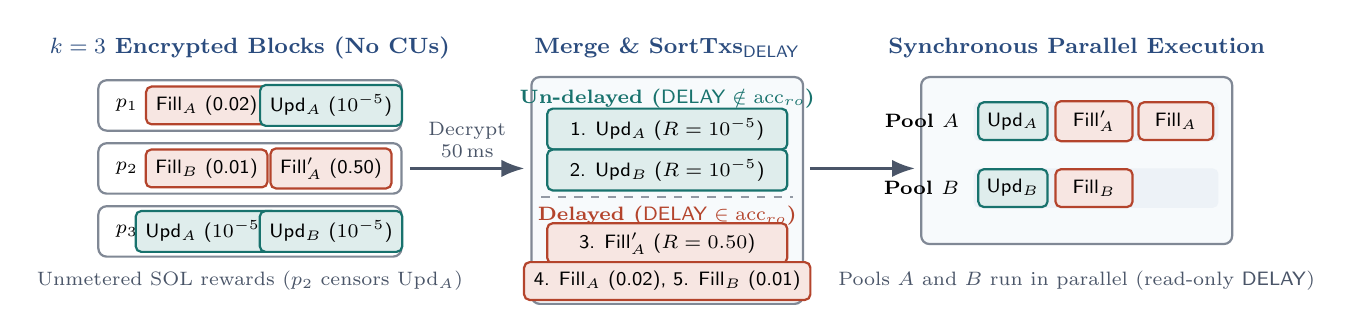
\begin{tikzpicture}[
  font=\footnotesize,
  >=Latex,
  box/.style={draw=slate!70, rounded corners=3pt, thick, fill=white, align=center},
  t0/.style={draw=tierzero!90!black, fill=tierzero!14, rounded corners=2pt, thick, minimum height=0.48cm, inner xsep=3.5pt, font=\scriptsize\sffamily},
  t1/.style={draw=tierone!90!black, fill=tierone!14, rounded corners=2pt, thick, minimum height=0.48cm, inner xsep=3.5pt, font=\scriptsize\sffamily}
]
\node[font=\footnotesize\bfseries, text=mcpblue] at (-0.15, 2.08) {$k=3$ Encrypted Blocks (No CUs)};
\node[box, minimum width=3.85cm, minimum height=0.64cm] at (-0.15, 1.35) {};
\node[anchor=west, font=\scriptsize\bfseries] at (-1.98, 1.35) {$p_1$};
\node[t1] at (-0.70, 1.35) {Fill$_A$ (0.02)};
\node[t0] at (0.88, 1.35) {Upd$_A$ ($10^{-5}$)};

\node[box, minimum width=3.85cm, minimum height=0.64cm] at (-0.15, 0.55) {};
\node[anchor=west, font=\scriptsize\bfseries] at (-1.98, 0.55) {$p_2$};
\node[t1] at (-0.70, 0.55) {Fill$_B$ (0.01)};
\node[t1] at (0.88, 0.55) {Fill$_A'$ (0.50)};

\node[box, minimum width=3.85cm, minimum height=0.64cm] at (-0.15, -0.25) {};
\node[anchor=west, font=\scriptsize\bfseries] at (-1.98, -0.25) {$p_3$};
\node[t0] at (-0.70, -0.25) {Upd$_A$ ($10^{-5}$)};
\node[t0] at (0.88, -0.25) {Upd$_B$ ($10^{-5}$)};
\node[font=\scriptsize, text=slate, align=center] at (-0.15, -0.88) {Unmetered SOL rewards ($p_2$ censors Upd$_A$)};

\node[font=\footnotesize\bfseries, text=mcpblue] at (5.15, 2.08) {Merge \& $\SortTxs_{\DelaySym}$};
\node[box, minimum width=3.45cm, minimum height=2.88cm, fill=softbg] at (5.15, 0.27) {};
\node[font=\scriptsize\bfseries, text=tierzero!90!black] at (5.15, 1.44) {Un-delayed ($\DelaySym \notin \mathrm{acc}_{ro}$)};
\node[t0, minimum width=3.05cm] at (5.15, 1.05) {1. Upd$_A$ ($R = 10^{-5}$)};
\node[t0, minimum width=3.05cm] at (5.15, 0.53) {2. Upd$_B$ ($R = 10^{-5}$)};
\draw[dashed, slate!60, thick] (3.55, 0.19) -- (6.75, 0.19);
\node[font=\scriptsize\bfseries, text=tierone!90!black] at (5.15, -0.05) {Delayed ($\DelaySym \in \mathrm{acc}_{ro}$)};
\node[t1, minimum width=3.05cm] at (5.15, -0.40) {3. Fill$_A'$ ($R = 0.50$)};
\node[t1, minimum width=3.05cm] at (5.15, -0.88) {4. Fill$_A$ (0.02), 5. Fill$_B$ (0.01)};

\node[font=\footnotesize\bfseries, text=mcpblue] at (10.35, 2.08) {Synchronous Parallel Execution};
\node[box, minimum width=3.95cm, minimum height=2.12cm, fill=softbg] at (10.35, 0.65) {};
\node[font=\scriptsize\bfseries, anchor=east] at (8.98, 1.15) {Pool $A$};
\fill[trackbg, rounded corners=2pt] (9.04, 0.90) rectangle (12.15, 1.40);
\node[t0, minimum width=0.88cm, inner xsep=2pt] at (9.54, 1.15) {Upd$_A$};
\node[t1, minimum width=0.98cm, inner xsep=2pt] at (10.57, 1.15) {Fill$_A'$};
\node[t1, minimum width=0.95cm, inner xsep=2pt] at (11.61, 1.15) {Fill$_A$};

\node[font=\scriptsize\bfseries, anchor=east] at (8.98, 0.30) {Pool $B$};
\fill[trackbg, rounded corners=2pt] (9.04, 0.05) rectangle (12.15, 0.55);
\node[t0, minimum width=0.88cm, inner xsep=2pt] at (9.54, 0.30) {Upd$_B$};
\node[t1, minimum width=0.98cm, inner xsep=2pt] at (10.57, 0.30) {Fill$_B$};
\node[font=\scriptsize, text=slate, align=center] at (10.35, -0.88) {Pools $A$ and $B$ run in parallel (read-only $\DelaySym$)};

\draw[->, very thick, slate] (1.88, 0.55) -- (3.34, 0.55) node[midway, above, font=\scriptsize, align=center] {Decrypt\\$50\,\text{ms}$};
\draw[->, very thick, slate] (6.96, 0.55) -- (8.30, 0.55);
\end{tikzpicture}%
}
\caption{One unmetered $50\,\text{ms}$ slot in $\NewCon + \DelaySym$. Although $\mathrm{cu}$ metering is removed and $p_2$ censors $\text{Upd}_A$ in favor of a $0.50\text{ SOL}$ sniper fill $\text{Fill}_A'$, $1$-of-$k$ inclusion via $p_1,p_3$ together with $K_{\text{unmetered}}$ executes $\text{Upd}_A$ first while Pool~$B$ executes concurrently.}
\label{fig:pipeline}
\end{figure}

\subsection{Asymmetric Account Enforcement and Atomic CPI Composability}

Enforcing the speed bump through $\DelaySym$ relies on a structural asymmetry in how Solana binds accounts to transactions.
\begin{itemize}[nosep,leftmargin=1.5em]
  \item \textbf{A maker can never be forced to include $\DelaySym$.} When updating a price, canceling an order, or executing a venue liquidation, the sender constructs and signs its own \texttt{UpdateQuote}, \texttt{Cancel}, or \texttt{Liquidate} transaction, cryptographically locking the transaction's account list, and writes directly to venue state without invoking untrusted external programs. Neither a proposer, a validator, nor a competing trader can inject $\DelaySym$ into the transaction, so these maker and exchange operations omit $\DelaySym$ and stay un-delayed ($\mathrm{delay}=0$).
  \item \textbf{A taker can always be forced to include $\DelaySym$.} To trade against a venue's liquidity, a taker must invoke the venue program's \texttt{Fill} (or \texttt{Take}) instruction, and the Solana runtime requires every account inspected anywhere in a transaction's CPI call graph to appear in the top-level transaction account list. When \texttt{Fill} verifies that one passed account has key $\DelaySym$ and reverts otherwise, every taker trade, including multi-hop aggregator routes and flash-loan bundles, is forced to list $\DelaySym \in \mathrm{acc}_{ro}(\mathit{tx})$ and execute as delayed ($\mathrm{delay}=1$).
\end{itemize}
For an instruction set $I(\mathit{tx})$, composition obeys $\mathrm{delay}(\mathit{tx}) = \max_{i \in I(\mathit{tx})} \mathrm{req}_{\DelaySym}(i)$. Unlike AMQs~\cite{CP25}, execution stays synchronous and atomic within one transaction; unlike generalized synchronous ACE~\cite{Can26}, multi-program calls never create conflicting permutations.

\section{Synergy with Multiple Concurrent Proposers}

A taker speed bump in $\SortTxs$ and concurrent block proposing close complementary halves of stale-quote sniping, as summarized in Table~\ref{tab:duality}.
\begin{itemize}[nosep,leftmargin=1.5em]
  \item \textbf{$\DelaySym$ without MCP degrades into censorship.} Under a single leader, a sniper who cannot sequence $\text{Fill}_A$ ahead of $\text{Upd}_A$ instead pays the leader $> R_u$ to omit $\text{Upd}_A$ from the slot~\cite{FPR23}.
  \item \textbf{MCP without $\DelaySym$ degrades into blind outbidding.} In \NewCon, $1$-of-$k$ inclusion~\cite[Thm.~2.2]{KW26c} lands $\text{Upd}_A$ and block hiding~\cite[Thm.~2.3]{KW26c} conceals it until blocks are fixed. Even so, a sniper seeing the same public price move can submit $\text{Fill}_A$ to any proposer and win whenever $R_f > (\mathrm{cu}_f/\mathrm{cu}_u) R_u$ (metered) or $R_f > R_u$ (unmetered).
\end{itemize}

\begin{proposition}[CU-Free Quote Precedence in $\NewCon + \DelaySym$]
\label{prop:synergy}
In an unmetered \NewCon{} slot $s$, suppose a maker sends a valid un-delayed update $\mathit{tx}_u$ ($\DelaySym \notin \mathrm{acc}_{ro}(\mathit{tx}_u)$, reward $R_u > 0$) to all $k$ proposers ($1$-of-$k$), and an adversary submits delayed fills $\{\mathit{tx}_f\}$ ($\DelaySym \in \mathrm{acc}_{ro}(\mathit{tx}_f)$) with arbitrary finite rewards $R_f$. In every non-skipped slot $s$ whose accepted proposer set $P_s$ contains at least one non-censoring proposer that received $\mathit{tx}_u$ in time, $\mathit{tx}_u$ executes strictly before every conflicting $\mathit{tx}_f$.
\end{proposition}

\begin{table}[h!]
\centering
\footnotesize
\renewcommand{\arraystretch}{1.16}
\begin{tabularx}{\textwidth}{@{}l Y Y Y@{}}
\toprule
\textbf{Architecture} & \textbf{Metered ($\mathrm{reward}/\mathrm{cu}$)} & \textbf{Unmetered ($\mathrm{reward}$ only)} & \textbf{Unmetered ($\DelaySym + \mathrm{reward}$)} \\
\midrule
\textbf{Single Leader}
  & Loose $\sim\!100\times$ fee cushion; leader can also censor update.
  & \textbf{Broken ($1\times$ cushion)} plus leader censorship.
  & \textbf{Vulnerable to censorship} once sniper bribe exceeds $R_u$. \\
\addlinespace[0.2em]
\textbf{\NewCon{} MCP}
  & Loose $\sim\!100\times$ cushion; public-signal jump snipes outbid update.
  & \textbf{Broken ($1\times$ cushion)} as any fill paying $> R_u$ snipes quote.
  & \textbf{CU-free speed bump} via $1$-of-$k$ inclusion and $\DelaySym$ ordering. \\
\bottomrule
\end{tabularx}
\caption{Removing $\mathrm{cu}$ metering requires $\DelaySym$ for maker priority, while $\DelaySym$ requires \NewCon's $1$-of-$k$ inclusion to prevent leader censorship.}
\label{tab:duality}
\end{table}

\section{Unmetered Solana Market Structure}

Each $50\,\text{ms}$ slot in $\NewCon + \DelaySym$ operates as a synchronous two-phase tick~\cite{BCS15,CF23}. Un-delayed transactions ($\DelaySym \notin \mathrm{acc}_{ro}$) first apply prop AMM \texttt{UpdateQuote} instructions, CLOB \texttt{Cancel} instructions, oracle pushes, and exchange \texttt{Liquidate} instructions collected across all $k$ proposers, after which delayed transactions ($\DelaySym \in \mathrm{acc}_{ro}$) execute speed-bumped \texttt{Fill} and \texttt{Take} instructions against fresh prices in the same slot (Table~\ref{tab:comparison}). Focused in-protocol taker speed bumps thus deliver the market-relevant core of ACE synchronously and atomically, allowing Solana to remove block $\mathrm{cu}$ limits, transaction $\mathrm{cu}$ limits, and runtime $\mathrm{cu}$ metering while preserving maker-friendly market structure.

\begin{table}[h!]
\centering
\footnotesize
\renewcommand{\arraystretch}{1.16}
\begin{tabularx}{\textwidth}{@{}l c c c c Y@{}}
\toprule
\textbf{ACE Approach} & \textbf{CU-Free?} & \textbf{Sync?} & \textbf{No Queue?} & \textbf{Atomic CPI?} & \textbf{Scope \& Tradeoff Without $\mathrm{cu}$ Metering} \\
\midrule
$\mathrm{reward}/\mathrm{cu}$ priority sort & \textbf{No} & Yes & Yes & Yes & Collapses to raw $\mathrm{reward}$ and $1\times R_u$ sniping \\
Async Market Queues~\cite{CP25} & Yes & \textbf{No} & \textbf{No} & \textbf{No} & General ACE, but queued, async, breaks CPI \\
Unanimity ordering~\cite{Can26} & Yes & Yes & Yes & Partial & General ACE, but cross-app conflicts revert to $\mathrm{reward}$ \\
\textbf{Taker speed bump (\DelayAcct{})} & \textbf{Yes} & \textbf{Yes} & \textbf{Yes} & \textbf{Yes} & \textbf{Focused speed bump with $1$-of-$k$ protection} \\
\bottomrule
\end{tabularx}
\caption{Comparison against Asynchronous Market Queues (AMQs)~\cite{CP25} and generalized in-protocol ACE~\cite{Can26}.}
\label{tab:comparison}
\end{table}

\begin{thebibliography}{KW26}\small\setlength{\itemsep}{2pt}\setlength{\parskip}{0pt}
\bibitem[BCS15]{BCS15}
E.~Budish, P.~Cramton, and J.~Shim. The high-frequency trading arms race and frequent batch auctions. \emph{Quarterly Journal of Economics}, 130(4), pp.~1547--1621, 2015.
\bibitem[Can26]{Can26}
A.~Canidio. Ordering by unanimity without breaking composability. \emph{arXiv preprint 2607.06144}, 2026.
\bibitem[CF23]{CF23}
A.~Canidio and R.~Fritsch. Batching trades on automated market makers. In \emph{5th ACM AFT}, 2023.
\bibitem[CP25]{CP25}
C.~Cool and J.~Pov\v{s}i\v{c}. Application Controlled Execution (ACE) through Asynchronous Market Queues (AMQs). Temporal Research, Sep.\ 2025. Code at \url{https://github.com/cavemanloverboy/ace}.
\bibitem[FPR23]{FPR23}
E.~Fox, M.~M. Pai, and M.~Resnick. Censorship resistance in on-chain auctions. In \emph{5th AFT}, LIPIcs 282, 2023.
\bibitem[KW26]{KW26c}
Q.~Kniep and R.~Wattenhofer. New Constellation, Multiple concurrent proposers for Alpenglow. Solana Foundation, v1.0, Nov.\ 14, 2026.
\end{thebibliography}

\end{document}
